\section{Modellierung der Burg}

\subsection{Grundaufbau der Burg}

Als die Vorüberlegungen abgeschlossen waren, musste möglichst schnell ein grundlegendes Modell der Burg geschaffen werden. Dieses Modell sollte alle überlegten Maße einhalten und somit als Erstfassung dienen, um in eine Unity Szene eingefügt werden zu können.

\begin{figure}[h]
	\centering
	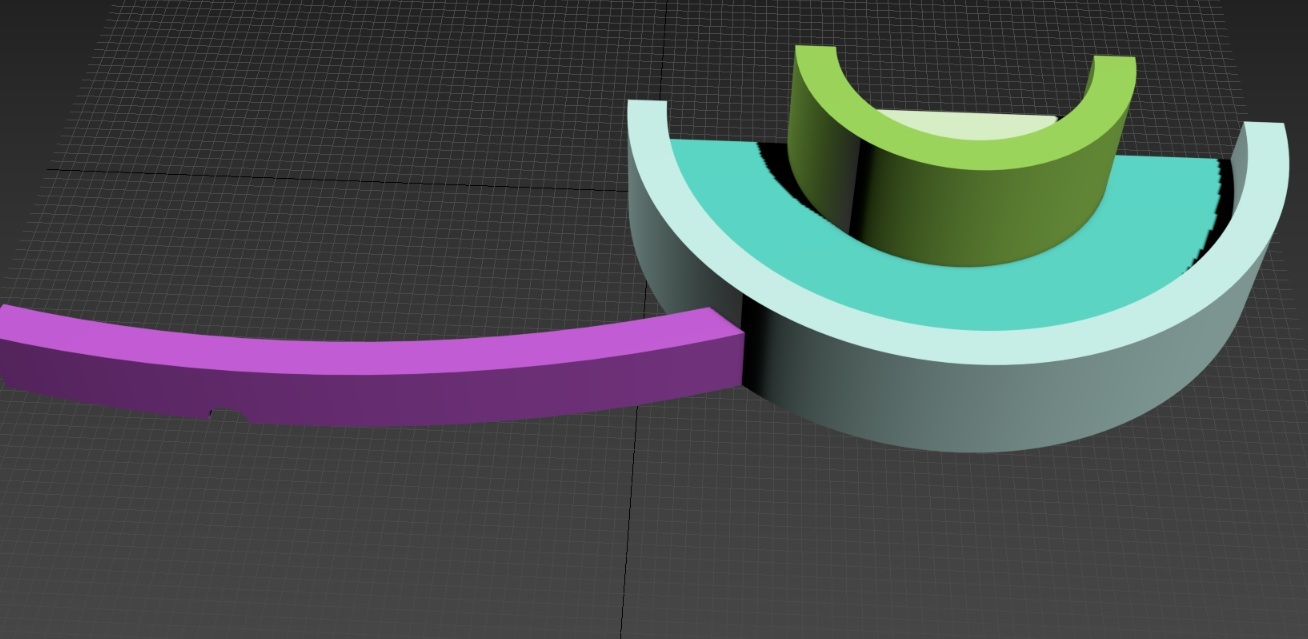
\includegraphics[width=0.95 \linewidth]{Abbildungen/3dsMax/Grundmodell}
	\caption{Grundaufbau der Burg}
	\label{fig:Grundaufbau}
\end{figure}

\begin{wrapfigure}{r}{0.5\textwidth}
	\begin{center}
		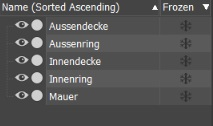
\includegraphics[width=0.45\textwidth]{Abbildungen/3dsMax/Grundhierachie}
	\end{center}
	\caption{Grundobjekte}
	\label{fig:Grundobjekte}
\end{wrapfigure}

Wie in den Abbildungen \ref{fig:Grundaufbau} und \ref{fig:Grundobjekte} zu sehen, besteht die Burg aus 5 Grundobjekten. Die Mauern wurden durch Röhren und die Decken durch Zylinder realisiert. Diese Objekte wurden anschließend in bearbeitbare Polys umgewandelt und zugeschnitten. Zum verschließen der daraus resultierenden offenen Enden wurde das Werkzeug \textit{Bridge} verwendet. Um später einen Fluss durch die lange Mauer fließen zu lassen, wurde unter Zuhilfenahme eines Zylinders und der boolschen Operation Subtrahieren eine halbrunde Öffnung hinzugefügt.

\newpage
\subsection{Modellierung des Haupttors}

\begin{figure}[h]
	\centering
	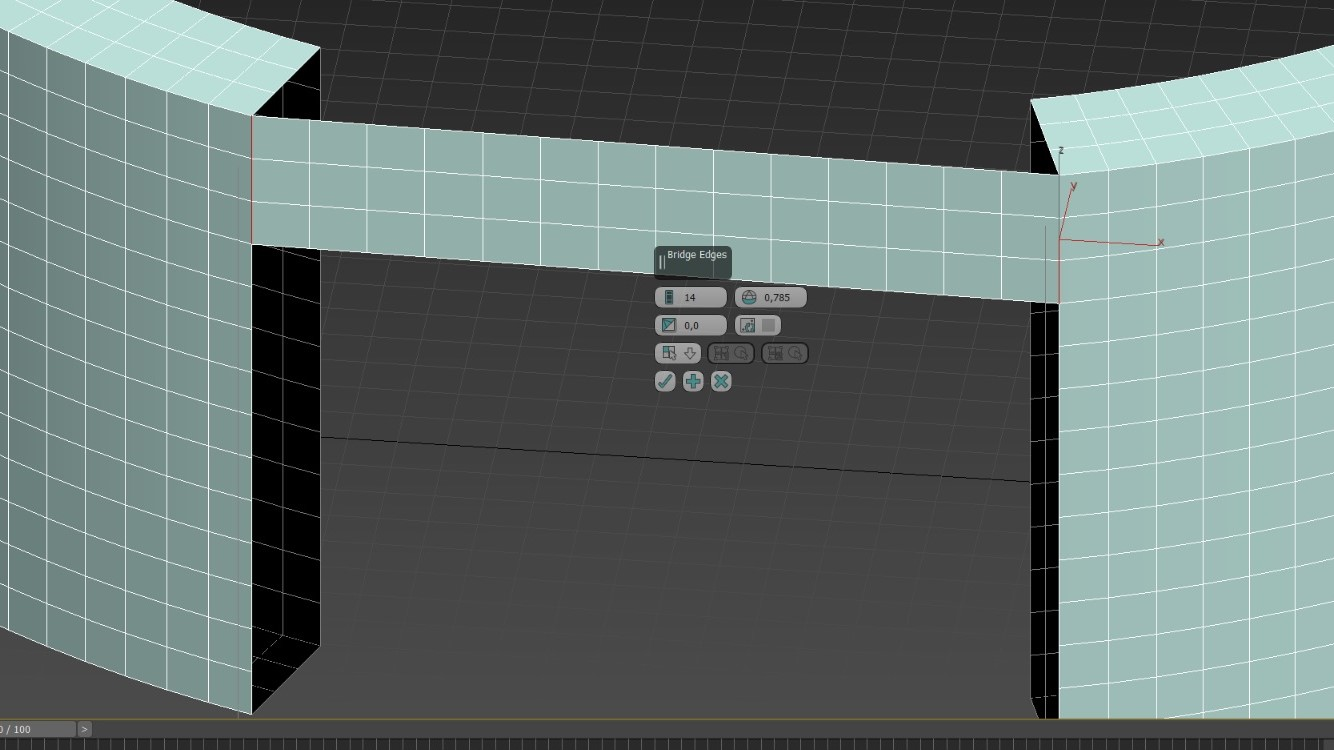
\includegraphics[width=0.95 \linewidth]{Abbildungen/3dsMax/Haupttor}
	\caption{Vorarbeit Haupttor}
	\label{fig:Haupttor}
\end{figure}

\begin{wrapfigure}{r}{0.5\textwidth}
	\begin{center}
		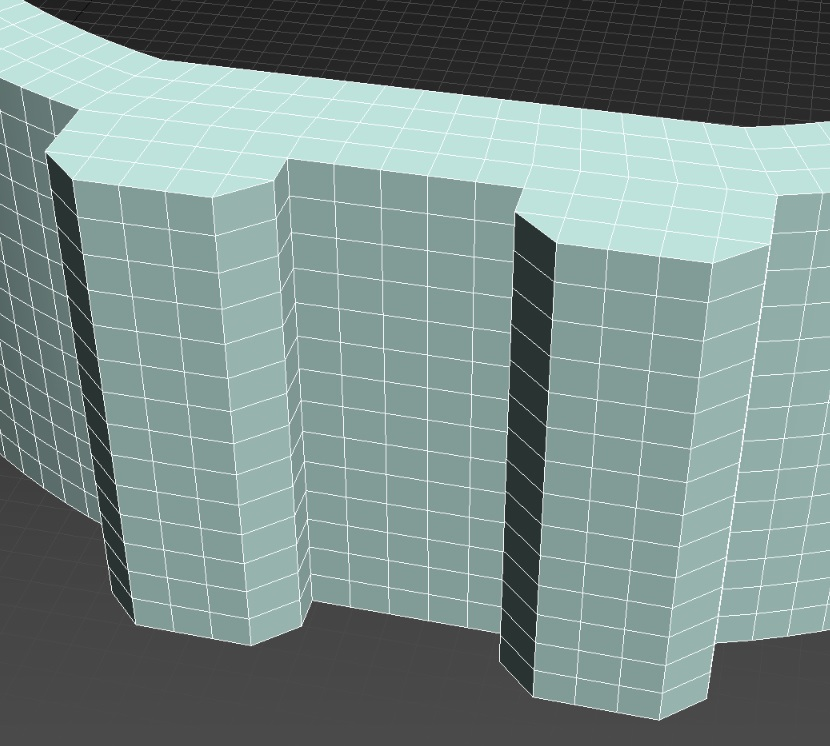
\includegraphics[width=0.45\textwidth]{Abbildungen/3dsMax/Haupttor2}
	\end{center}
	\caption{Haupttor}
	\label{fig:Haupttor2}
\end{wrapfigure}



Der nächste Schritt umfasste die Modellierung des Haupttores. Um eine gerade Arbeitsfläche zu erhalten, wurde der Mittelteil des Außenrings herausgeschnitten. Die nun freilegenden Kanten wurden, wie in Abb. \ref{fig:Haupttor} zu sehen mit dem \textit{Bridge} Werkzeug verbunden. Die Türme des Tores wurden anschließend mit dem \textit{Extrude} Werkzeug herausgearbeitet. Wie in Abb. \ref{fig:Haupttor2} zu sehen sind die frontalen Ecken der Türme "abgeschnitten". Um dies zu erreichen gibt es in 3dsMax verschiedene Möglichkeiten. In diesem Fall wurde das Kantenwerkzeug \textit{Chamfer} benutzt. Dies erlaubt es Ecken durch automatisches hinzufügen neuer Kanten abzurunden. Um das gewünschte Ziel zu erreichen wurde die Kantenanzahl verdoppelt.

\newpage
\subsection{Treppenbau}

\begin{figure}[h]
	\centering
	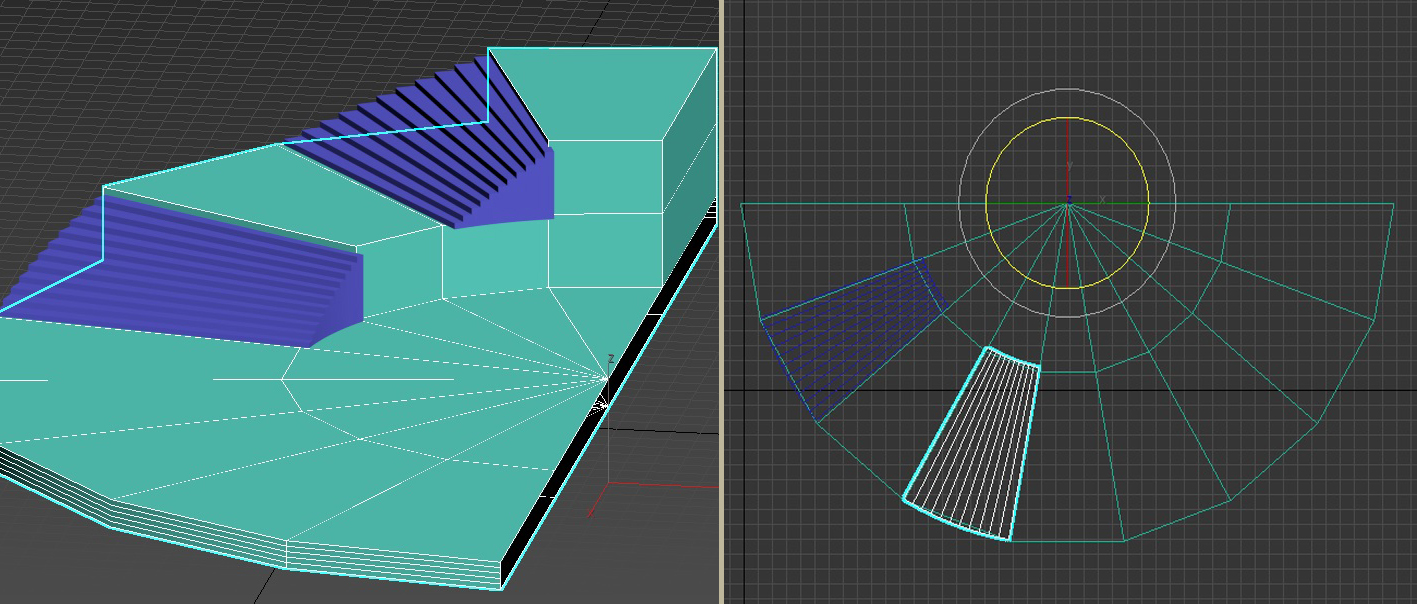
\includegraphics[width=0.95 \linewidth]{Abbildungen/3dsMax/Treppe_final}
	\caption{Treppenbau}
	\label{fig:Treppe}
\end{figure}

\begin{wrapfigure}{r}{0.3\textwidth}
	\begin{center}
		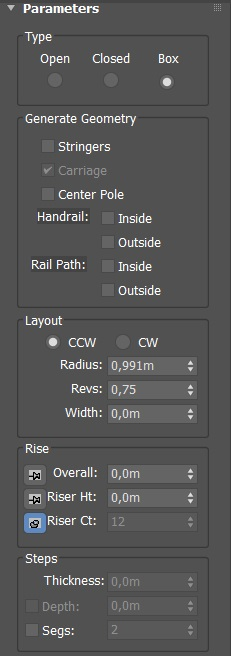
\includegraphics[width=0.25\textwidth]{Abbildungen/3dsMax/Treppe3}
	\end{center}
	\caption{Treppenparameter}
	\label{fig:Parameter}
\end{wrapfigure}

Um den erhöhten Innenring zu erreichen, musste eine Möglichkeit gefunden werden den Höhenunterschied auszugleichen. Treppen waren das Mittel der Wahl. Dazu wurde, wie in Abb. \ref{fig:Treppe} links zu sehen, die Außendecke mit dem\textit{Extrude} Befehl angepasst. Über die 3dsMax Objektauswahl können direkt Treppen als Grundobjekte erstellt werden. Da die Treppen in eine Rundung eingepasst werden sollten, wurden die \textit{SpiralStairs} gewählt. Abb. \ref{fig:Parameter} zeigt einen Ausschnitt der zu modifizierenden Parameter. Um einen geschlossenen Treppenkörper zu erhalten, wurde \textit(Box) gewählt. Der Radius der Treppe gleicht dem der Außendecke, um eine genaue Einpassung zu ermöglichen. Die Treppe wurde nun , wie in Abb. \ref{fig:Treppe} rechts gesehen, so verschoben, dass der Pivot Punkt der Treppe, dem der Außendecke entspricht. Um Sicherzustellen das später der First Person Controller die Treppen erklimmen kann, wurde darauf geachtet, dass Stufenhöhe und -tiefe Maßen entsprechen, welche auch in der Realität Anwendung finden. Dies ermöglichte der Parameter \textit{Riser Ht}, der zwischen 20cm - 30cm gewählt wurde. Auch im weiteren Modellierungsprozess wurden vermehrt Treppen eingesetzt, um die Begehung der Burg spannender zu gestalten.

\newpage
\subsection{Verfeinerung der Mauern}

\begin{figure}[h]
	\centering
	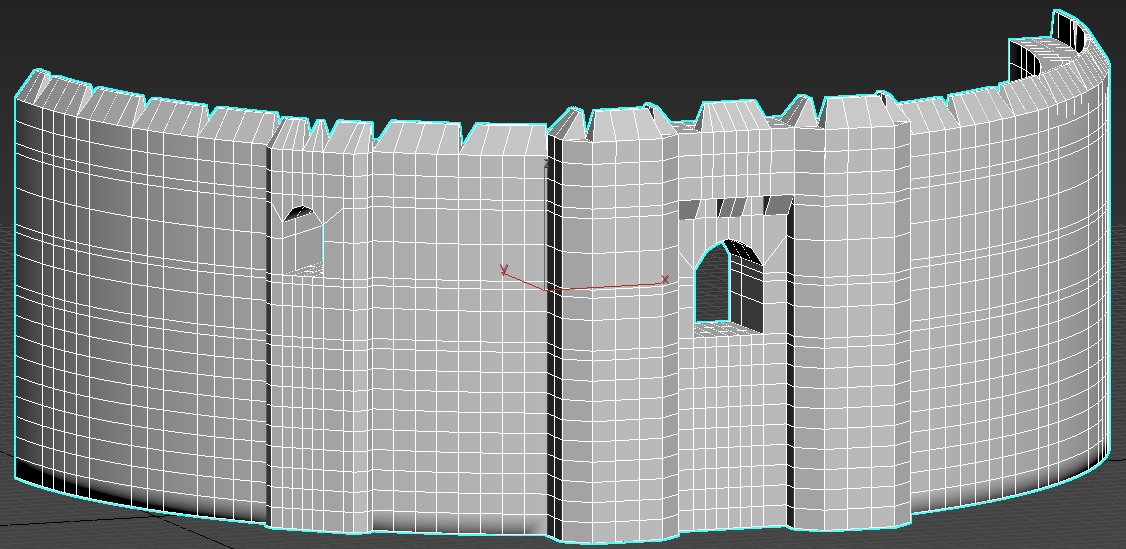
\includegraphics[width=0.95 \linewidth]{Abbildungen/3dsMax/Aussenring}
	\caption{Verfeinerung Außenring}
	\label{fig:Aussenring}
\end{figure}

Um den Außenring detaillierter zu gestalten, wurden hauptsächlich die Polygonwerkzeuge \textit{Extrude} und \textit{Bevel} genutzt. Durch paarweises auswählen und \textit{Bevel} wurden die Zinnen herausgearbeitet. Auch die obere Seite des Haupttores wurde mittels \textit{Extrude} detaillierter gestaltet. Um die Toröffnung herauszuarbeiten, wurden mithilfe des Kantenauswahlwerkzeugs \textit{Ring} alle horizontalen Kanten ausgewählt und mittels \textit{Connect} neue vertikale Kanten eingefügt. Durch gezieltes verschieben von Eckpunkten wurde die obere Rundung geforrmt. Der Durchgang wurde durch löschen der Polygone geschaffen und die daraus resultierenden offenen Fläche mithilfe des \textit{Bridge} Werkzeugs geschlossen. 

\begin{figure}[h]
	\centering
	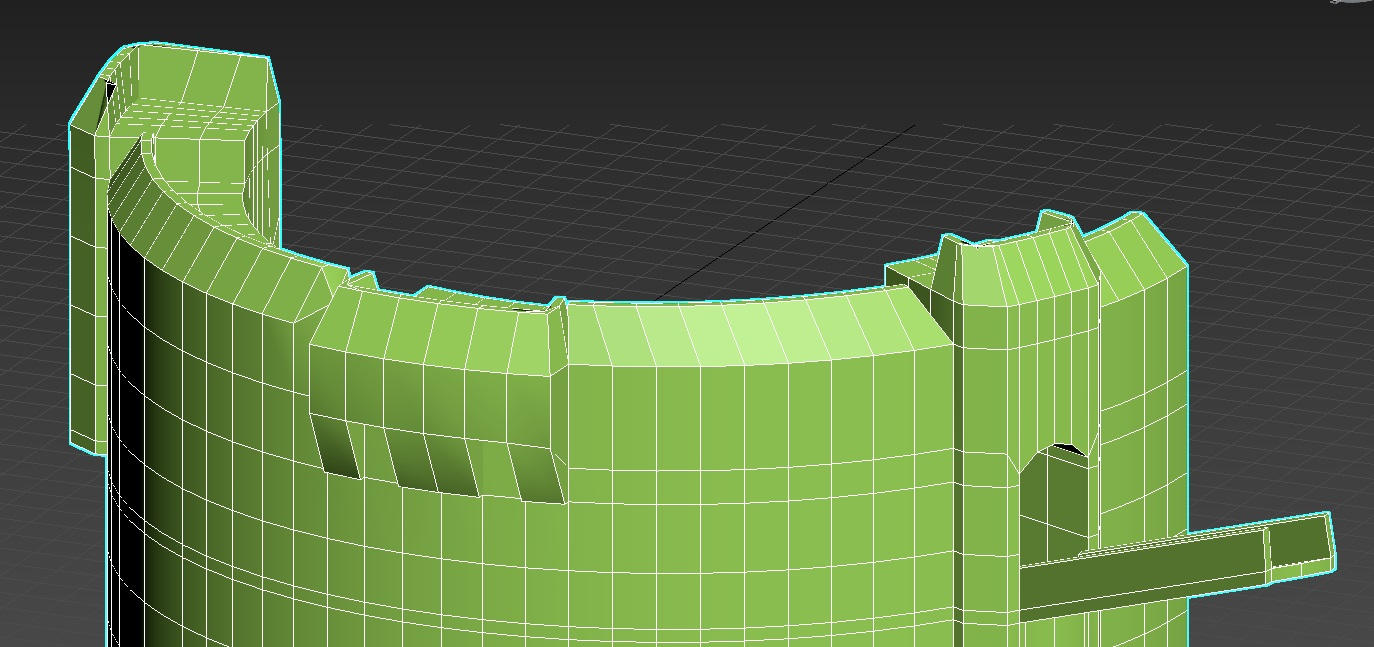
\includegraphics[width=0.95 \linewidth]{Abbildungen/3dsMax/Innenring}
	\caption{Verfeinerung Innenring}
	\label{fig:Innenring}
\end{figure}

Wie in Abb. \ref{fig:Innenring} zu sehen, wurde der Innenring ähnlich zum Außenring gestaltet, um einen einheitlichen Gesamteindruck zu erhalten. Die Zinnen sind aber ohne Schießscharten gehalten. Zum Abschluss wurde noch durch den \textit{Extrude} Befehl eine Brücke zum erreichen des Außenrings angefügt.

\begin{figure}[h]
	\centering
	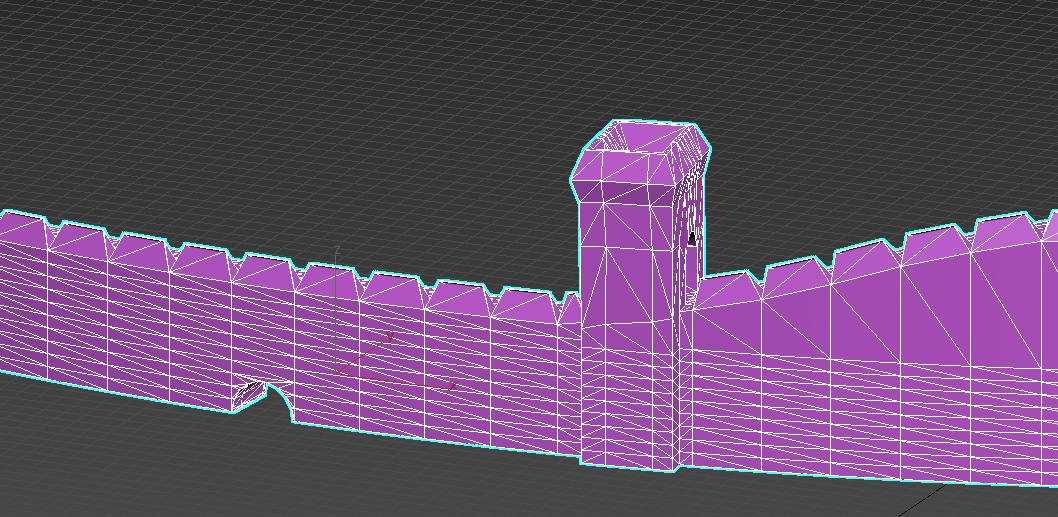
\includegraphics[width=0.95 \linewidth]{Abbildungen/3dsMax/Mauer}
	\caption{Verfeinerung Mauer}
	\label{fig:Mauer}
\end{figure}

Abb. \ref{fig:Mauer} zeigt die lange Verteidigungsmauer und den bereits erwähnten Flussdurchgang. Auch hier wurden Zinnen herausgearbeitet und des weiteren ein Wachturm mit Durchgang angefügt.
\newpage

\subsection{Haupthaus und Turm}

\begin{figure}[h]
	\centering
	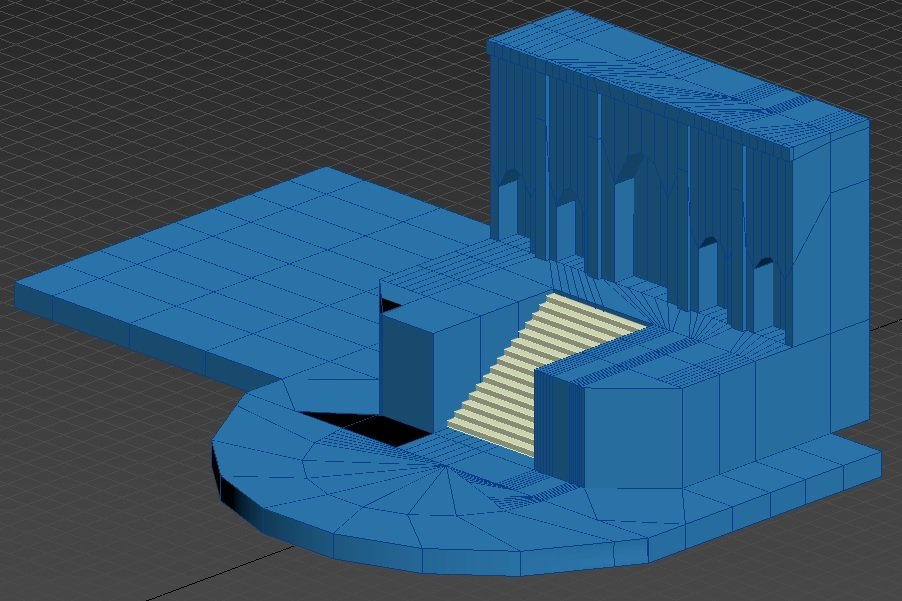
\includegraphics[width=0.95 \linewidth]{Abbildungen/3dsMax/Gebaeude}
	\caption{Haupthaus}
	\label{fig:Haupthaus}
\end{figure}

\begin{wrapfigure}{r}{0.3\textwidth}
	\begin{center}
		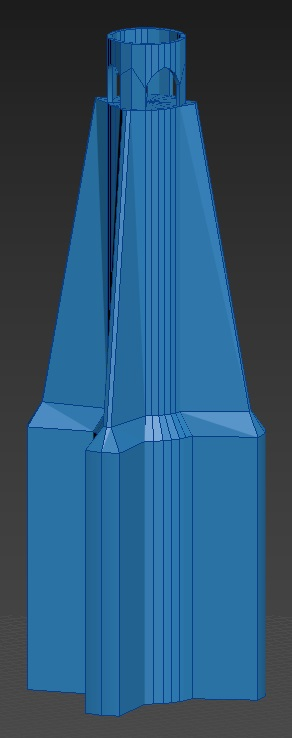
\includegraphics[width=0.22\textwidth]{Abbildungen/3dsMax/Turm}
	\end{center}
	\caption{Turm}
	\label{fig:Turm}
\end{wrapfigure}

Um Platz für das in Abb. \ref{fig:Haupthaus} zu sehende Haupthaus zu schaffen, wurde die halbrunde Innendecke mit mehrfachem Einsatz des \textit{Extrude} Befehls erweitert. Auch eine Plattform für den in Abb. \ref{fig:Turm} zu sehenden Turm wurde geschaffen. Der Turm besteht aus einem Zylinder, welcher durch das \textit{Extrude} und \textit{Bevel} Werkzeug in die gewünschte Form gebracht wurde. Ähnlich der Durchgänge, wurden Aussparungen am oberen Teil des Turmes angebracht.
\newpage

\subsection{Texturierung der Burg}

\begin{figure}[h]
	\centering
	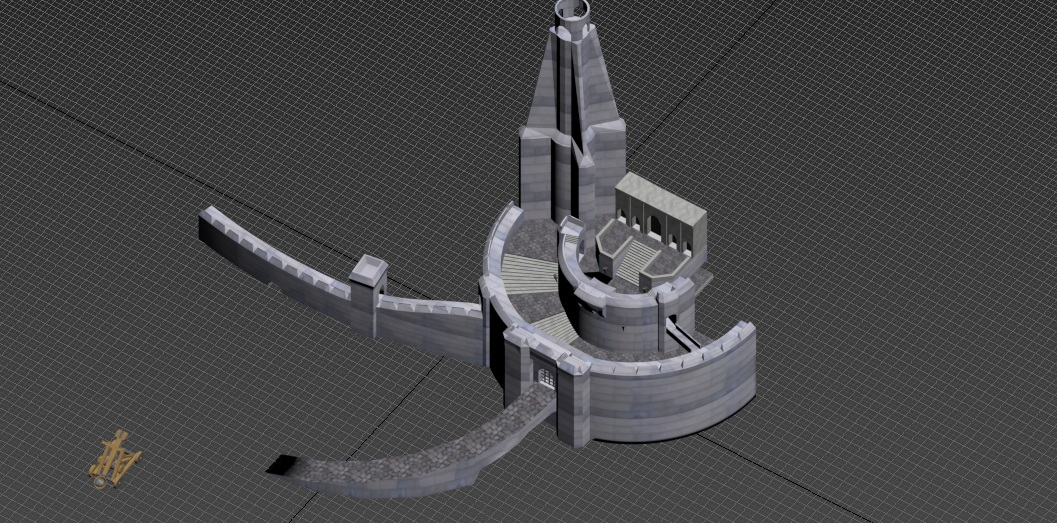
\includegraphics[width=0.95 \linewidth]{Abbildungen/3dsMax/Burg_final}
	\caption{texturierte Burg}
	\label{fig:Burg_final}
\end{figure}
 